\documentclass{article}
\usepackage[utf8]{inputenc}
\usepackage{graphicx}
\usepackage{amsmath}

\title{Homework Set 8 - PHYS 728 Radio Astronomy}
\author{Matthew Cooper}
\date{April 10th, 2019}
\begin{document}
\begin{titlepage}
\maketitle
\end{titlepage}

\textbf{Problem 8.1-Solution}:

\smallskip
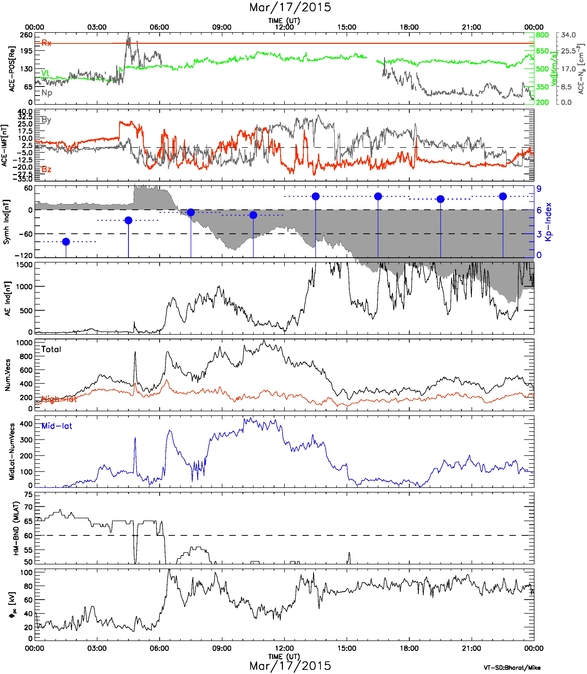
\includegraphics[scale=2.2]{/media/matthew/64EC-62D6/RadioAstronomy/Homework8-Natey/geoMagneticActivity.jpg}

a.)  From panel 3 of the above plot, the SSC occured at around 4:50 am.  Sudden storm commencement is when a strong pulse of solar wind from the sun strikes the magnetosphere.  This shocks the magnetosphere, leading to a temporarily increased magnetic field, which quickly lessens as the ring current starts building up.

b.)  The ring current hits its maximum around 23:00 hours, since the symmetric magnetic field is strongest at this point, which can be seen from panel 3 as well.

c.)  The highest number of vectors occurred from 11:00-12:00 hours, as can be seen from panels 5 and 6.

d.)  The magnetic potential spikes concurrently with the sudden storm onset, which is seen in panel 8.

\pagebreak
\textbf{Problem 8.2-Solution}:

\smallskip
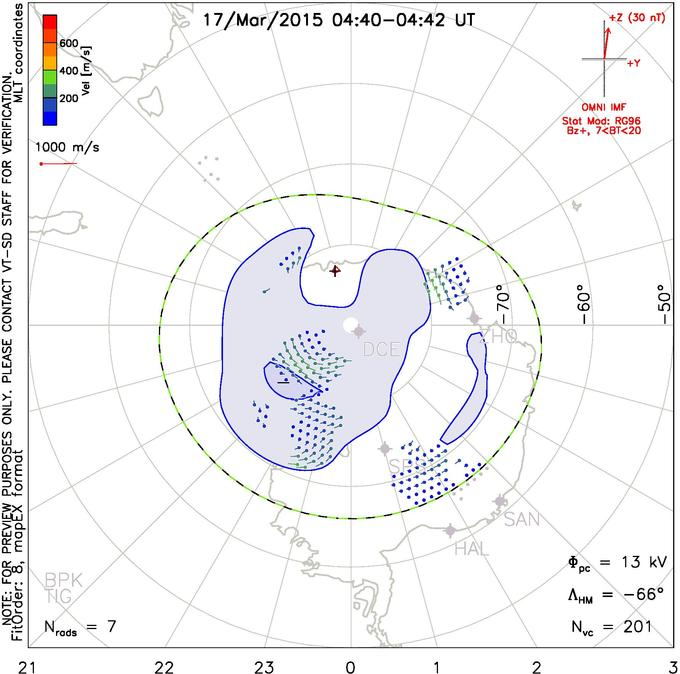
\includegraphics[scale=1]{/media/matthew/64EC-62D6/RadioAstronomy/Homework8-Natey/onset10BeforeSouth.jpg}
\smallskip
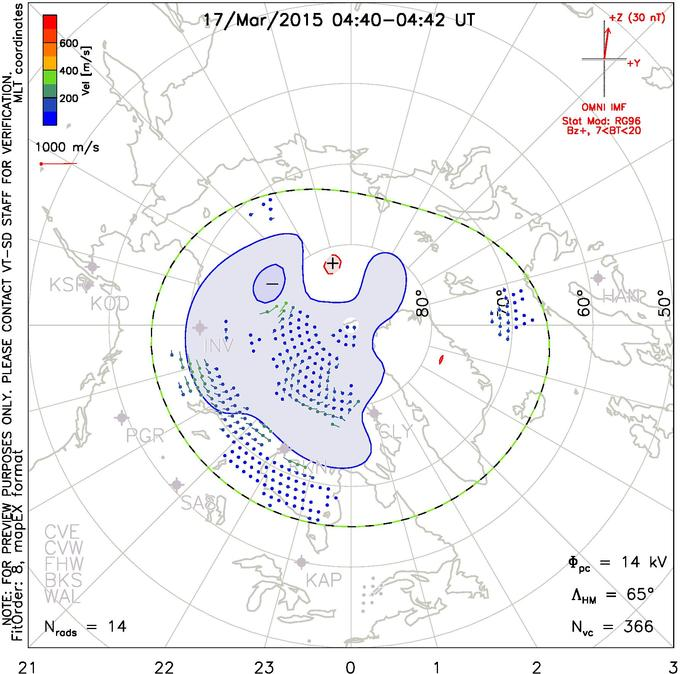
\includegraphics[scale=1]{/media/matthew/64EC-62D6/RadioAstronomy/Homework8-Natey/onset10BeforeNorth.jpg}

\smallskip
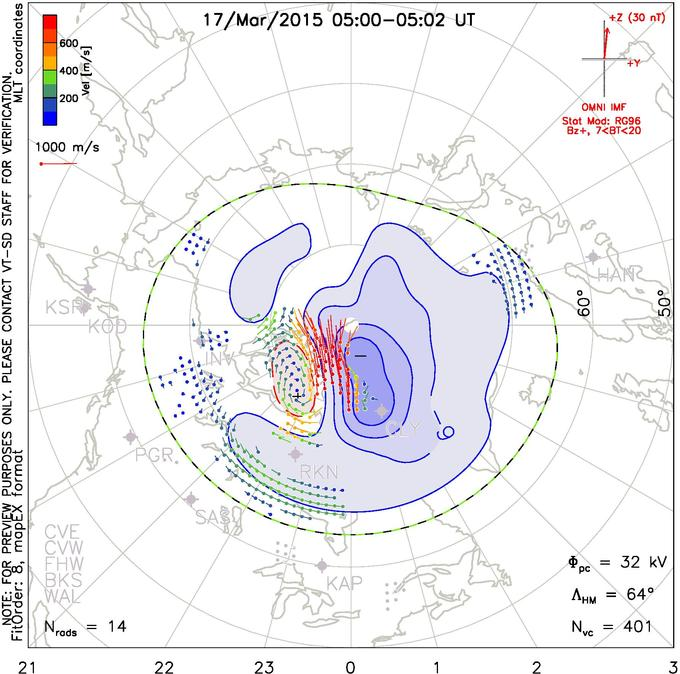
\includegraphics[scale=1]{/media/matthew/64EC-62D6/RadioAstronomy/Homework8-Natey/onset10AfterNorth.jpg}
\smallskip
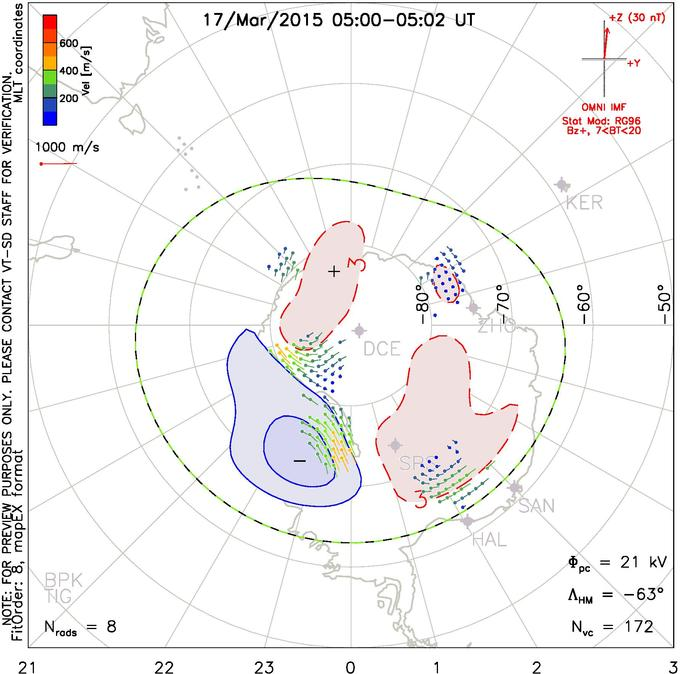
\includegraphics[scale=1]{/media/matthew/64EC-62D6/RadioAstronomy/Homework8-Natey/onset10AfterSouth.jpg}

a.) Before the abrupt increase in the magnetic potential, the convection seems relatively calm.  After the onset, there is significantly faster convection and turbulence.  This could be a result of magnetic reconnection at the bow shock propagating around to the tail, affecting the convection of the ionosphere and above.

b.) Before the onset, the Northern and Souther Hemispheres look quite similar.  Afterward, in the Northern Hemisphere, there is a very localized high speed region, while in the Southern Hemisphere there appears to be less localization of the effect.

\pagebreak
\textbf{Problem 8.3-Solution}:

\smallskip
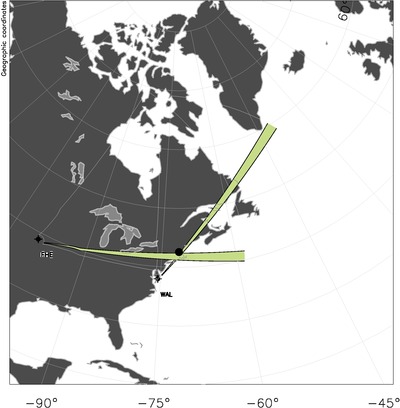
\includegraphics[scale=3]{/media/matthew/64EC-62D6/RadioAstronomy/Homework8-Natey/MillstoneHillCoverage.png}

For Millstone Hill, there are two beams that cover the area, one from Wallops Island, Beam 11, which has a ground range of 619 km, and one from Fort Hayes East, Beam 19, which has a ground range of 2381 km.

\pagebreak
\textbf{Problem 8.4-Solution}:

a.) The data gets very sparse after 1200 UT.

\smallskip
b.) Yes, the other beams would be beneficial in order to provide context of the surrounding atmospheric convection which is contributing to the measurements being taken by the ISR.  It would also help if the ISR was not at a relatively high inclination, since the beam from the ISR might cross other beam paths during measurements.
\end{document}